\documentclass{article}

\usepackage{tikz}
\usetikzlibrary{positioning}
\usetikzlibrary{arrows}
\usetikzlibrary{automata,positioning}

\usepackage{stmaryrd}

\newcommand{\imp}{\rightarrow}
\newcommand{\biimp}{\leftrightarrow}
\newcommand{\all}{\forall}
\newcommand{\ex}{\exists}
\newcommand{\seq}{\vdash}
\newcommand{\nec}{\Box} % necessarily
\newcommand{\pos}{\Diamond} % possibly
\newcommand{\ess}[2]{#1 \ \mathit{ess.} \ #2}
\newcommand{\NE}{\mathit{NE}}




\usepackage{a4wide,hyperref,fancyvrb,amsmath,amssymb,graphicx}
\DefineShortVerb{\+}

\title{A Universal Logic Theorem Proving Approach \\ \large ---San Francisco, Feb 20,
  2016---}
\author{Christoph Benzm\"uller}
\date{}


\begin{document}
\maketitle

This draft document, which I have produced in a rush, is available at
\href{http://www.christoph-benzmueller.de/2016-SFO/tutorial.pdf}{http://www.christoph-benzmueller.de/2016-SFO/tutorial.pdf};
please forgive any 
typos, errors, trivialities, etc. 

\section{(Before the tutorial starts) Installing Isabelle}
The Isabelle proof assistant is available at
\href{https://isabelle.in.tum.de/}{https://isabelle.in.tum.de/}.
There you also find various tutorials and documentations. The Isabelle
system should ideally be installed before the tutorial starts, since
this will take a while. Everything else below can be download and
installed on the fly.

\section{First Steps: Quantified Modal Logics}
\subsection{Install Convenient Abbreviations for Logic Embedding}
Download the file
\href{http://www.christoph-benzmueller.de/2016-SFO/Isabelle/abbrevs}{http://www.christoph-benzmueller.de/2016-SFO/Isabelle/abbrevs}
and store it on your computer at +~/.isabelle/Isabelle2016/jedit/abbrevs+.

In a shell you may simply do this as follows: \\[1em]
+ cd ~/.isabelle/Isabelle2016/jedit/+ \\
+ mv abbrevs abbrevs.save.1+\\
+ wget http://www.christoph-benzmueller.de/2016-SFO/Isabelle/abbrevs+
\\[1em]
Now go to +Isabelle2016>Preferences>Abbreviations+  
and activate +Space bar expands abbrevs+. Then klick +Apply+ and +OK+.

By this procedure you have activated the following, very convenient abbreviations for
entering connectives in the embedding approach (which are displayed in Isabelle in
boldface). In order to enable their display you need to
hit +space+ after entering the shortcuts.\\[1em]

\begin{tabular}{l|l|l}
shortcut & alternative latex-like input & displayed as \\ \hline
+mneg+ & +\bol\not+ & $\boldsymbol{\neg}$ \\
+mor+ & +\bol\or+ & $\boldsymbol{\vee}$ \\
+mand+ & +\bol\and+ & $\boldsymbol{\wedge}$ \\
+mimpl+ & +\bol\right+ & $\boldsymbol{\rightarrow}$ \\
+mequiv+ & +\bol\leftr+ & $\boldsymbol{\leftrightarrow}$ \\
+mall+ & +\bol\for+ & $\boldsymbol{\forall}$ \\
+mexi+ & +\bol\exi+ & $\boldsymbol{\exists}$ \\
+mnegpred+ &  & ${^\neg}$ \\
+mvalid+ &  +\lf\rf+ & ${\lfloor}\, {\rfloor}$ \\
\end{tabular}

\subsection{Download the Logic Embedding of Quantified Modal Logic}
Create a working directory and change the directory accordingly. Then
download the Isabelle file
\href{http://www.christoph-benzmueller.de/2016-SFO/Isabelle/QML.thy}{http://www.christoph-benzmueller.de/2016-SFO/Isabelle/QML.thy} \\[1em]
+ mkdir ~/LogicEmbeddingsTutorial+ \\
+ cd ~/LogicEmbeddingsTutorial+\\
+ wget http://www.christoph-benzmueller.de/2016-SFO/Isabelle/QML.thy+\\[1em]
You may also want to download the following example file: \\
\href{http://www.christoph-benzmueller.de/2016-SFO/Isabelle/QMLex1.thy}{http://www.christoph-benzmueller.de/2016-SFO/Isabelle/QMLex1.thy} 
\\[1em]
+ wget http://www.christoph-benzmueller.de/2016-SFO/Isabelle/QMLex1.thy+


\subsection{Inspect the Encoding of the Logic Embedding}
Start Isabelle and open file +QML.thy+ (+File>Open>QML.thy>Open+).
Read and inspect the file (see Fig~\ref{QML.thy}); try to understand the embedding
(explanations will be given in classroom). Related information can be
found here: 
\begin{itemize}
\item Quantified Multimodal Logics in Simple Type Theory, In Logica Universalis (Special Issue
  on Multimodal Logics), volume 7, number 1, pp. 7-20, 2013. Available
  \href{http://christoph-benzmueller.de/papers/J23.pdf}{http://christoph-benzmueller.de/papers/J23.pdf}.
\item Slides: \href{http://christoph-benzmueller.de/papers/2015-Tableaux.pdf}{http://christoph-benzmueller.de/papers/2015-Tableaux.pdf}
   \href{http://christoph-benzmueller.de/papers/2016-Berkeley.pdf}{http://christoph-benzmueller.de/papers/2016-Berkeley.pdf}
%  (coming soon)
\end{itemize}

\begin{figure}[t]
\centerline{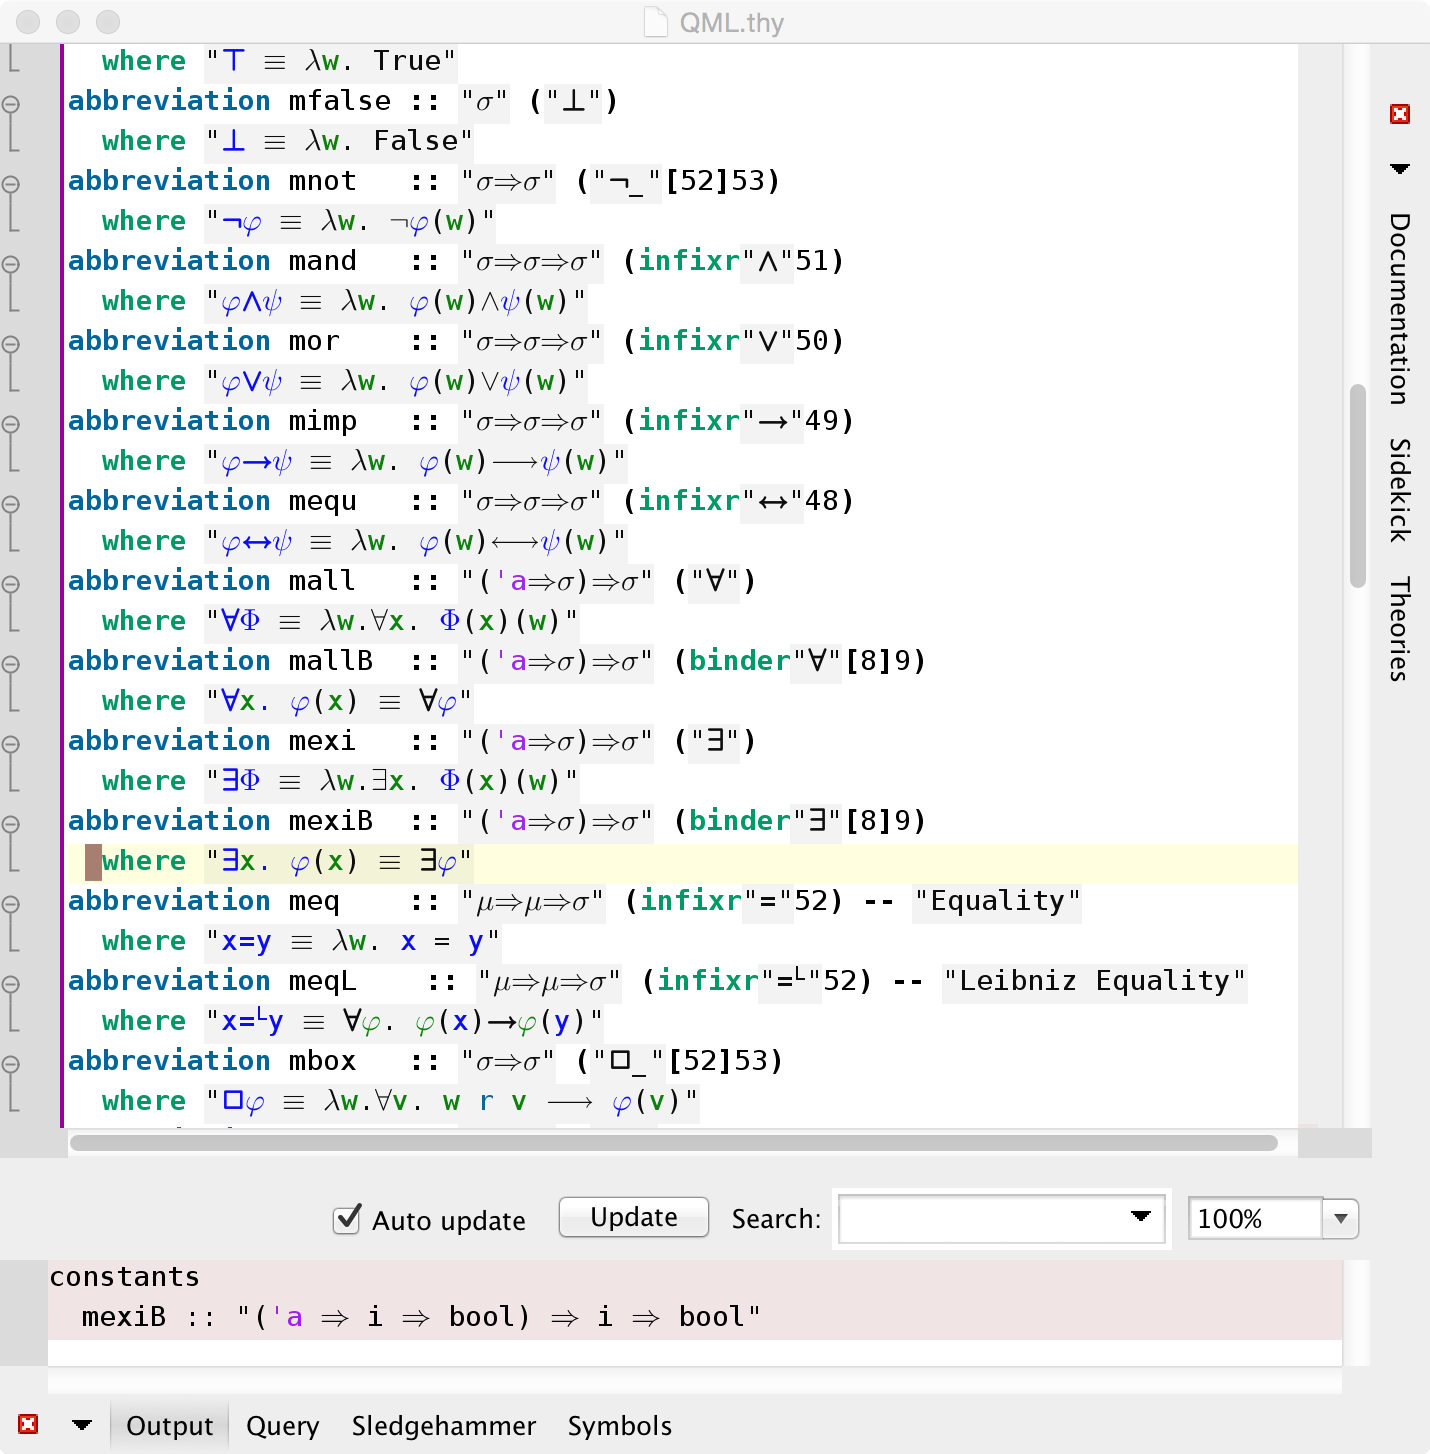
\includegraphics[width=.7\columnwidth]{./Images/QML.png}}
\caption{File QML.thy} \label{QML.thy}
\end{figure}

\subsection{Entering Formulas and Proving Them}
In this part of the tutorial we will get familiar with theorem proving in
Isabelle/HOL. Our focus will be on proof automation with tools inbuilt
to Isabelle and with external reasoners. However, we will also briefly
address interactive theorem proving in the Isar proof language. Here
are some useful texts for studying:
\begin{itemize}
\item Hammering Away --
A User’s Guide to Sledgehammer for Isabelle/HOL (Jasmin Christian
Blanchette), 2015. Available here
\href{http://isabelle.in.tum.de/dist/doc/sledgehammer.pdf}{http://isabelle.in.tum.de/dist/doc/sledgehammer.pdf}.
\item Nitpick: A Counterexample Generator for Isabelle/HOL Based on
  the Relational Model Finder Kodkod (Jasmin Christian Blanchette),
  2013. Available \href{http://www.easychair.org/publications/paper/Nitpick_A_Counterexample_Generator_for_Isabelle_HOL_Based_on_the_Relational_Model_Finder_Kodkod}{\textbf{here}}.
\item The Isabelle/Isar Reference Manual (Makarius Wenzel),
  2015. \\
Available at \href{http://isabelle.in.tum.de/doc/isar-ref.pdf}{http://isabelle.in.tum.de/doc/isar-ref.pdf}.
\end{itemize}


During the tutorial we will inspect some of the examples in file
+QMLex1.png+ (see Fig.\ref{QMLex1}).
\begin{figure}[t]
\centerline{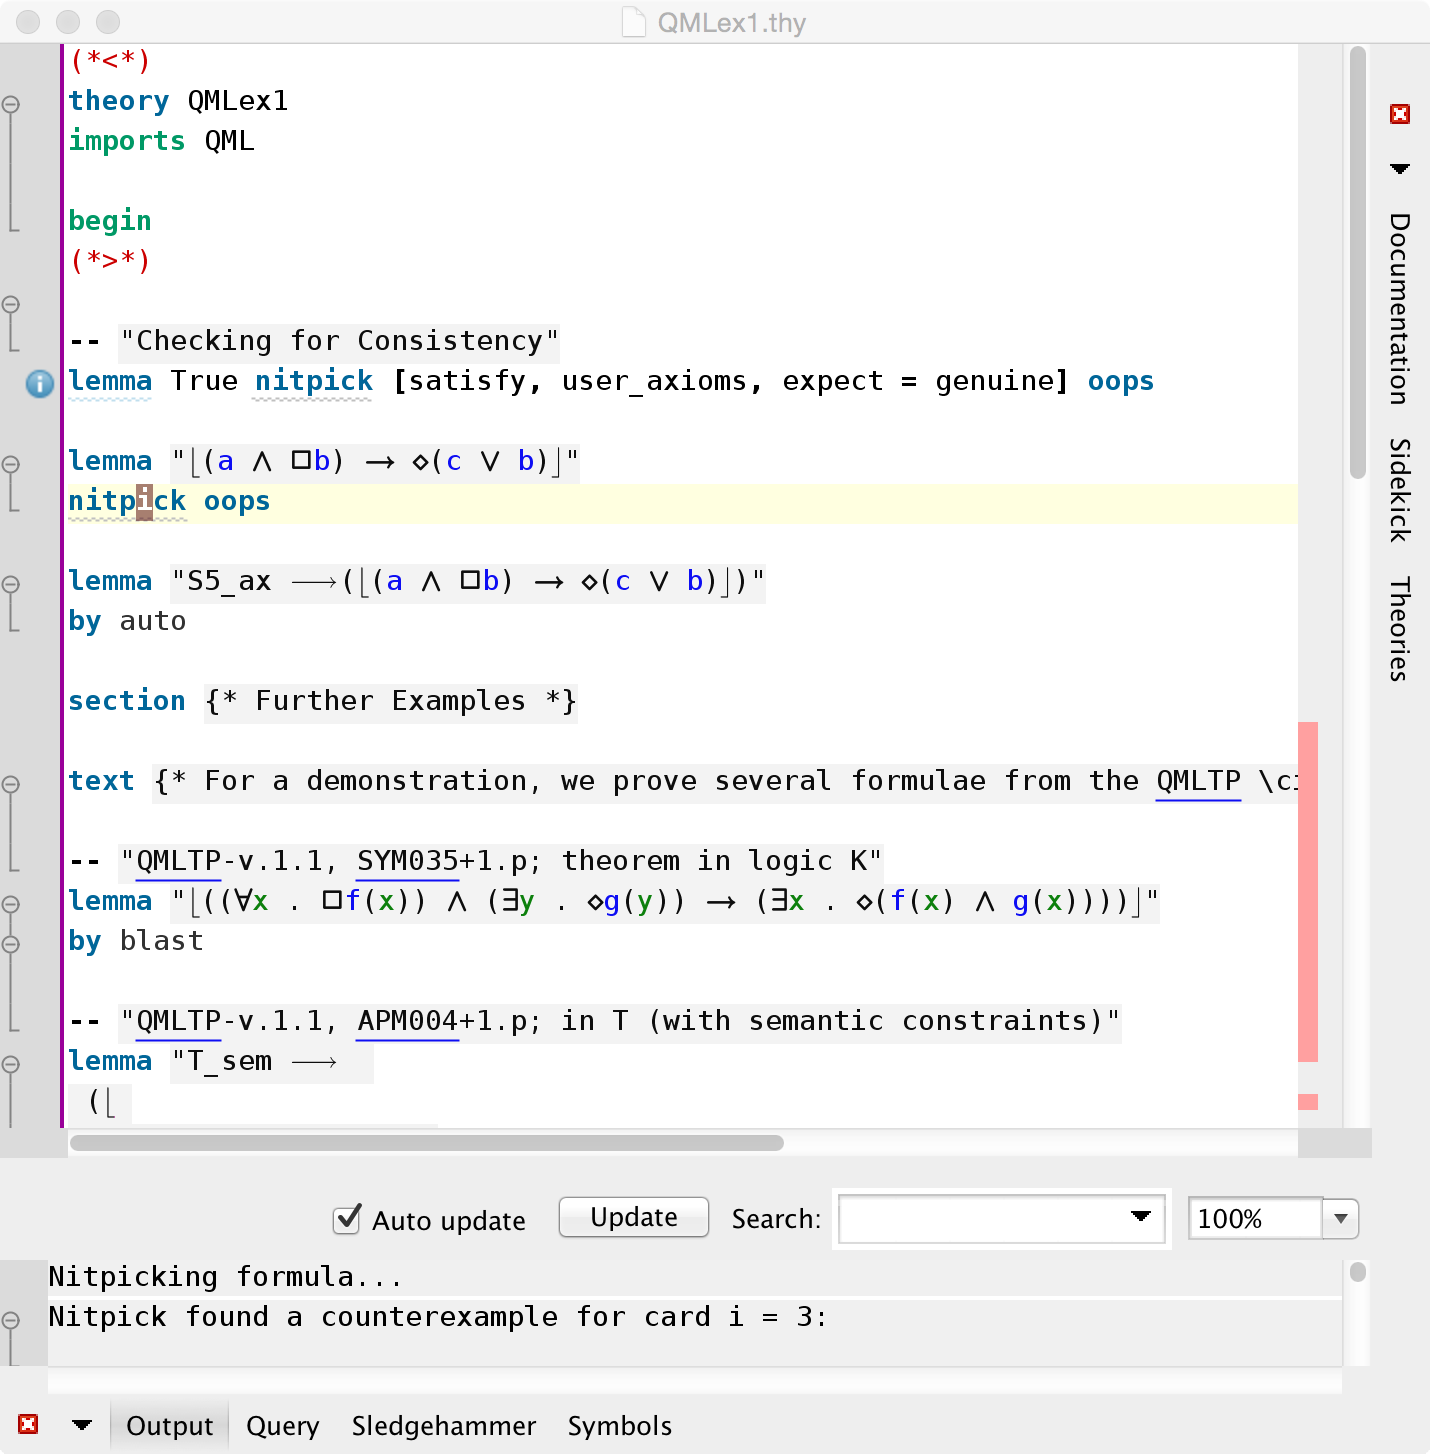
\includegraphics[width=.7\columnwidth]{./Images/QMLex1.png}}
\caption{File QMLex1.thy} \label{QMLex1}
\end{figure}

\subsubsection{Exercise}
Make up some little toy examples in propositional, first-order or
higher-order modal logic with pen and paper and subsequently
encode them in Isabelle/HOL utilising the semantic embedding provided in 
file +QML.ax+. Try to prove them with Sledgehammer or disprove them
with Nitpick.

\subsubsection{Exercise}
Encode instances of the Barcan Formula ($\forall x. \square F(x)
\longrightarrow \Box \forall x. F(x)$; domains cannot grow) and the Converse Barcan
Formula ($\Box \forall x. F(x) \longrightarrow \forall x. \Box F(x)$; domains cannot shrink)
and study their validity within Isabelle/HOL utilising the semantic
embedding approach. Try to prove them with Sledgehammer or disprove them
with Nitpick.


\subsubsection{Exercise}
Encode the propositions 3.2, 3.3, 4.2, and 5.2 from the
following paper:
\begin{itemize}
\item Can Modalities Save Naive Set Theory? (Peter Fritz, Harvey
  Lederman, Tiankai Liu and Dana Scott), 2015 (draft). Available at \href{http://logic.berkeley.edu/colloquium/ScottModalPaper.pdf}{http://logic.berkeley.edu/colloquium/ScottModalPaper.pdf}
\end{itemize}
Prove them automatically using the embedding approach in Isabelle/HOL.



\section{Meta-logical Reasoning}

\subsection{Verification of the Modal Logic Cube}
In this part of the tutorial we discuss an automated verification of
the well-known modal logic cube (see Fig.~\ref{cube})
in Isabelle/HOL, in which we prove the
inclusion relations between the cube’s logics using automated
reasoning tools. Prior work addresses this problem but without
restriction to the modal logic cube, and using encodings in
first-order logic in combination with first-order automated theorem
provers. In contrast, our solution is more elegant, transparent and
effective. It employs the introduced embedding of quantified modal logic in
classical higher-order logic. Automated reasoning tools, such as
Sledgehammer with LEO-II, Satallax and CVC4, Metis and Nitpick, are
employed to achieve full automation. Though successful, the
experiments also motivate some technical improvements in the
Isabelle/HOL tool.


\begin{figure}[t]
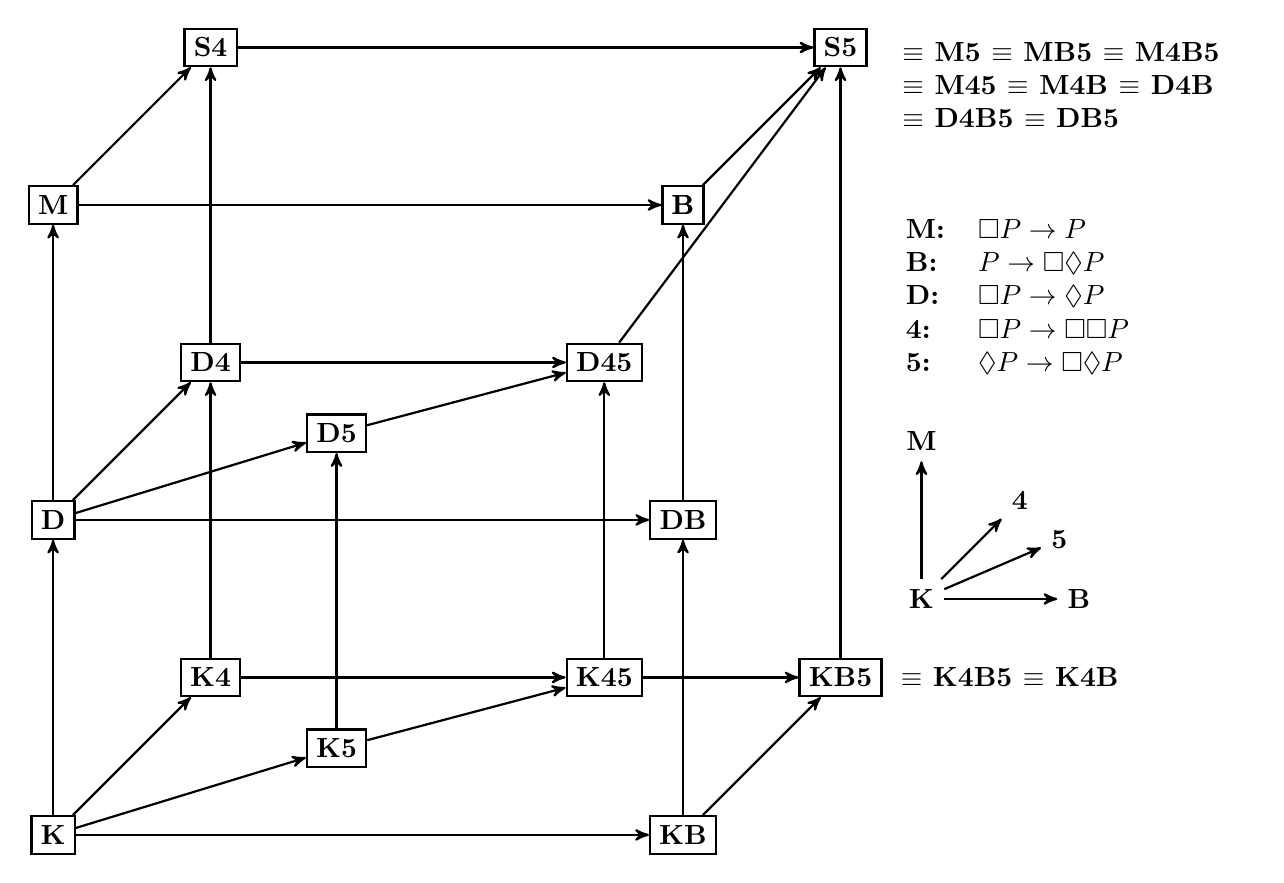
\begin{tikzpicture}[thick,node/.style={rectangle,draw,font=\normalsize\bfseries}]

  % 1. Ebene
  \node[node] (K)   {K};
  \node[node] (K4)  [above right=2cm and 2cm of K.center,anchor=center] {K4};
  \node[node] (K5)  [below right=0.9cm and 1.6cm of K4.center,anchor=center] {K5};
  \node[node] (KB)  [right=8cm of K.center,anchor=center] {KB};
  \node[node] (K45) [right=5cm of K4.center,anchor=center] {K45};
  \node[node] (KB5) [above right=2cm and 2cm of KB.center,anchor=center] {KB5};

  % 2. Ebene
  \node[node] (D)  [above=4cm of K.center,anchor=center] {D};
  \node[node] (D4) [above right=2cm and 2cm of D.center,anchor=center] {D4};
  \node[node] (D5) [below right=0.9cm and 1.6cm of D4.center,anchor=center] {D5};
  \node[node] (DB) [right=8cm of D.center,anchor=center] {DB};
  \node[node] (D45)[right=5cm of D4.center,anchor=center] {D45};

  % 3. Ebene
  \node[node] (M)  [above=4cm of D.center,anchor=center] {M};
  \node[node] (S4) [above right=2cm and 2cm of M.center,anchor=center] {S4};
  \node[node] (B)  [right=8cm of M.center,anchor=center] {B};
  \node[node] (B)  [right=8cm of M.center,anchor=center] {B};
  \node[node] (S5) [above right=2cm and 2cm of B.center,anchor=center] {S5};

  \node[align=center,font=\normalsize\bfseries] [right=0.1cm of S5.north east,anchor=north west]
   {\begin{tabular}{ l }
     $\equiv$ M5 $\equiv$ MB5 $\equiv$ M4B5\\
     $\equiv$ M45 $\equiv$ M4B $\equiv$ D4B\\
     $\equiv$ D4B5 $\equiv$ DB5
    \end{tabular}
    };
  \node[align=left,font=\normalsize\bfseries] [above right=1.75cm and 3cm of D45.north east,anchor=north west]
   {
   \begin{tabular}{ l l }
      M: & $\nec P \rightarrow P$ \\
      B: & $P \rightarrow \nec\pos P$ \\
      D: & $\nec P \rightarrow \pos P$ \\
      4: & $\nec P \rightarrow \nec\nec P$ \\
      5: & $\pos P \rightarrow \nec\pos P$
   \end{tabular}
   };

  \node[draw=none,fill=none,font=\normalsize\bfseries] (K1) [below right=2.5cm and 3.25cm of D45.south east,anchor=north west] {K};
  \node[draw=none,fill=none,font=\normalsize\bfseries] (M1) [above=2cm of K1.center,anchor=center] {M};
  \node[draw=none,fill=none,font=\normalsize\bfseries] (41) [above right=1.25cm and 1.25cm of K1.center,anchor=center] {4};
  \node[draw=none,fill=none,font=\normalsize\bfseries] (51) [above right=0.75cm and 1.75cm of K1.center,anchor=center] {5};
  \node[draw=none,fill=none,font=\normalsize\bfseries] (B1) [right=2cm of K1.center,anchor=center] {B};
   
  \node[align=center,font=\normalsize\bfseries] [right=0.1cm of KB5.north east,anchor=north west]
   {$\equiv$ K4B5 $\equiv$ K4B};
  \path[->,>=stealth',thick,every node/.style={font=\large}]
    (K1)  edge (M1)
          edge (41)
          edge (51)
          edge (B1);

  \path[->,>=stealth',thick,every node/.style={font=\large}]
    (K)   edge (K4)
          edge (K5)
          edge (KB)
          edge (D)
    (K4)  edge (K45)
          edge (D4)
    (K5)  edge (K45)
          edge (D5)
    (KB)  edge (KB5)
          edge (DB)
    (K45) edge (KB5)
          edge (D45)
    (KB5) edge (S5)

    (D)   edge (D4)
          edge (D5)
          edge (DB)
          edge (M)
    (D4)  edge (D45)
          edge (S4)
    (D5)  edge (D45)
    (DB)  edge (B)
    (D45) edge (S5)

    (M)  edge (S4)
         edge (B)
    (S4) edge (S5)
    (B)  edge (S5);
    
\end{tikzpicture}
\caption{Modal Logic Cube} \label{cube}
\end{figure}

Here is some further material on this work
\begin{itemize}
\item Systematic Verification of the Modal Logic Cube in Isabelle/HOL
  (Christoph Benzm\"uller, Maximilian Claus, Nik Sultana), In PxTP 2015, EPTCS, volume 186,
  pp. 27-41, 2015. Available at
  \href{http://christoph-benzmueller.de/papers/C47.pdf}{http://christoph-benzmueller.de/papers/C47.pdf}
\item Slides at:  \href{http://christoph-benzmueller.de/papers/2015-PxTP.pdf}{http://christoph-benzmueller.de/papers/2015-PxTP.pdf}
\item Isabelle source files: 
\href{http://www.christoph-benzmueller.de/2016-SFO/Isabelle/mcube-final.zip}{http://www.christoph-benzmueller.de/2016-SFO/Isabelle/mcube-final.zip} 
\end{itemize}
+ cd ~/LogicEmbeddingsTutorial+\\
+ mkdir ModalCube+ \\
+ cd ModalCube+ \\
+ wget http://www.christoph-benzmueller.de/2016-SFO/Isabelle/mcube-final.zip+ \\
+ unzip mcube-final.zip+ \\
+ cd mcube+ \\
+ ls+ \\[1em]
You will find the file +ModalCube.thy+. We will discuss the content of
this file in the tutorial. Feel free to play with it!


\subsection{Exercise}
Prove in Isabelle that the following options to axiomatise modal logic
S5 are all equivalent.  S5: M5 $\Leftrightarrow$ MB5 $\Leftrightarrow$
M4B5 $\Leftrightarrow$ M45 $\Leftrightarrow$ M4B $\Leftrightarrow$ D4B
$\Leftrightarrow$ D4B5 $\Leftrightarrow$ DB5. Try it with the semantic
and the syntactic version of the respective axioms.



\subsection{Demo of the Isabelle-build Tool}
We will demonstrate how LaTeX quality
publications can be produced directly from Isabelle source documents. \\[1em]
+ cd ~/LogicEmbeddingsTutorial/ModalCube/mcube+\\
+ /Applications/Isabelle2015.app/Isabelle/bin/isabelle build -D .+ \\
+ open ~/LogicEmbeddingsTutorial/ModalCube/mcube/doc/document.pdf+
\\[1em]


\section{Intuitionistic Logic}

\subsection{G\"odel Translation}
We combine G\"odels interpretation of propositional
intuitionistic logic in propositional modal logic S4 with our above
embedding in order to provide a sound and complete embedding of propositional intuitionistic logic into HOL.

Further reading:
\begin{itemize}
\item Multimodal and Intuitionistic Logics in Simple Type Theory
  (Christoph Benzm\"uller, Lawrence Paulson), In The Logic Journal of
  the IGPL, Oxford University Press, volume 18, number 6, pp. 881-892,
  2010. Available at:
  \href{http://christoph-benzmueller.de/papers/J21.pdf}{http://christoph-benzmueller.de/papers/J21.pdf}
\item Eine Interpretation des Intuitionistischen Aussagenkalk\"uls (Kurt G\"odel),  Ergebnisse eines Mathematischen Kolloquiums, 8:39–40, 1933.
\end{itemize}
The relevant files are \\[1em]
+ cd ~/LogicEmbeddingsTutorial+\\
+ mkdir IntuitionisticLogic+ \\
+ cd IntuitionisticLogic+ \\
+ wget http://www.christoph-benzmueller.de/2016-SFO/Isabelle/Intuitionistic.thy+
\\

We will discuss the content of this file during the tutorial.

\subsection{Exercise}
Analyse the validity resp. countersatisfiability of the Law of
Excluded Middle, Double Negation Elimination, the Law
of Contradiction and Ex Falso Quodlibet in Isabelle.

\subsubsection{Exercise}
Make up your own examples in propositional intuitionistic logic and try to prove or refute them in Isabelle.

\subsubsection{Exercise}
Remove axiom S4 in file +Intuitionistic.thy+ and identify and report
the changes regarding the investigated principles in that file.

\subsubsection{Exercise}
Add further connectives and quantifiers to the file
+Intuitionistic.thy+, so that we obtain a corresponding embedding of
quantified intuitionistic logic in HOL.

\subsubsection{Exercise}
Make up your own examples in quantified intuitionistic logic and try to prove or refute them in Isabelle.


\subsection{McKinsey-Tarski Translation}
A slightly different mapping of propositional intuitionistic logic
into modal logic S4 has been proposed by McKinsey and Tarski.
\begin{itemize}
\item McKinsey, J. C. C.; Tarski, Alfred. Some Theorems About the Sentential Calculi of Lewis and Heyting. J. Symbolic Logic 13 (1948), no. 1, 1--15.
\end{itemize}
You find this embedding in the second half of file
+Intuitionistic.thy+. 

\subsubsection{Exercise}
Analyse the validity resp. countersatisfiability of the Law of
Excluded Middle, Double Negation Elimination, the Law
of Contradiction and Ex Falso Quodlibet in Isabelle.

\subsubsection{Exercise}
Analyse the equivalence of both embeddings in Isabelle.



\section{The Ontological Argument}
Kurt G\"odel's ontological argument for God's existence has been
formalized and automated on a computer with higher-order automated
theorem provers. From G\"odel's premises, the computer proved:
necessarily, there exists God. On the other hand, the theorem provers
have also confirmed prominent criticism on G\"odel's ontological
argument, and they found some new results about it.

In this part of the tutorial we will analyse variants of the
Ontological Argument with HOL ATPs.

Here is some further material on this work
\begin{itemize}
\item Automating G\"odel's Ontological Proof of God's Existence with
Higher-order Automated Theorem Provers (Christoph Benzm\"uller, Bruno
Woltzenlogel Paleo), In ECAI 2014 (Torsten Schaub, Gerhard Friedrich,
Barry O'Sullivan, eds.), IOS Press, Frontiers in Artificial
Intelligence and Applications, volume 263, pp. 93 -- 98,
2014. Available at:   \href{http://christoph-benzmueller.de/papers/C40.pdf}{http://christoph-benzmueller.de/papers/C40.pdf}
\item Invited Talk: On a (Quite) Universal Theorem Proving Approach and Its Application in Metaphysics (Christoph Benzm\"uller), In TABLEAUX 2015 (Hans De Nivelle, ed.), Springer, LNAI, volume 9323, pp. 209-216, 2015. Available at:   \href{http://christoph-benzmueller.de/papers/C50.pdf}{http://christoph-benzmueller.de/papers/C50.pdf}
\item Slides from my UC Berkeley talk at:
  \href{http://christoph-benzmueller.de/papers/2015-Berkeley.pdf}{http://christoph-benzmueller.de/papers/2015-Berkeley.pdf}
 %  (coming soon)
\end{itemize}

First we download some files to be studied to be reused in the
subsections below:\\[1em]
+ cd ~/LogicEmbeddingsTutorial+\\
+ mkdir OntologicalArgument+ \\
+ cd OntologicalArgument+ \\
+ wget http://www.christoph-benzmueller.de/2016-SFO/Isabelle/QML.thy+\\
+ wget http://www.christoph-benzmueller.de/2016-SFO/Isabelle/Scott.thy+  \\

\subsection{Scott's Variant}
The file +Scott.thy+ contains Dana Scott's version of G\"odel's ontological
argument (see Fig.~\ref{Scott.thy}). We will discuss the content in classroom.

\begin{figure}[t]
\centerline{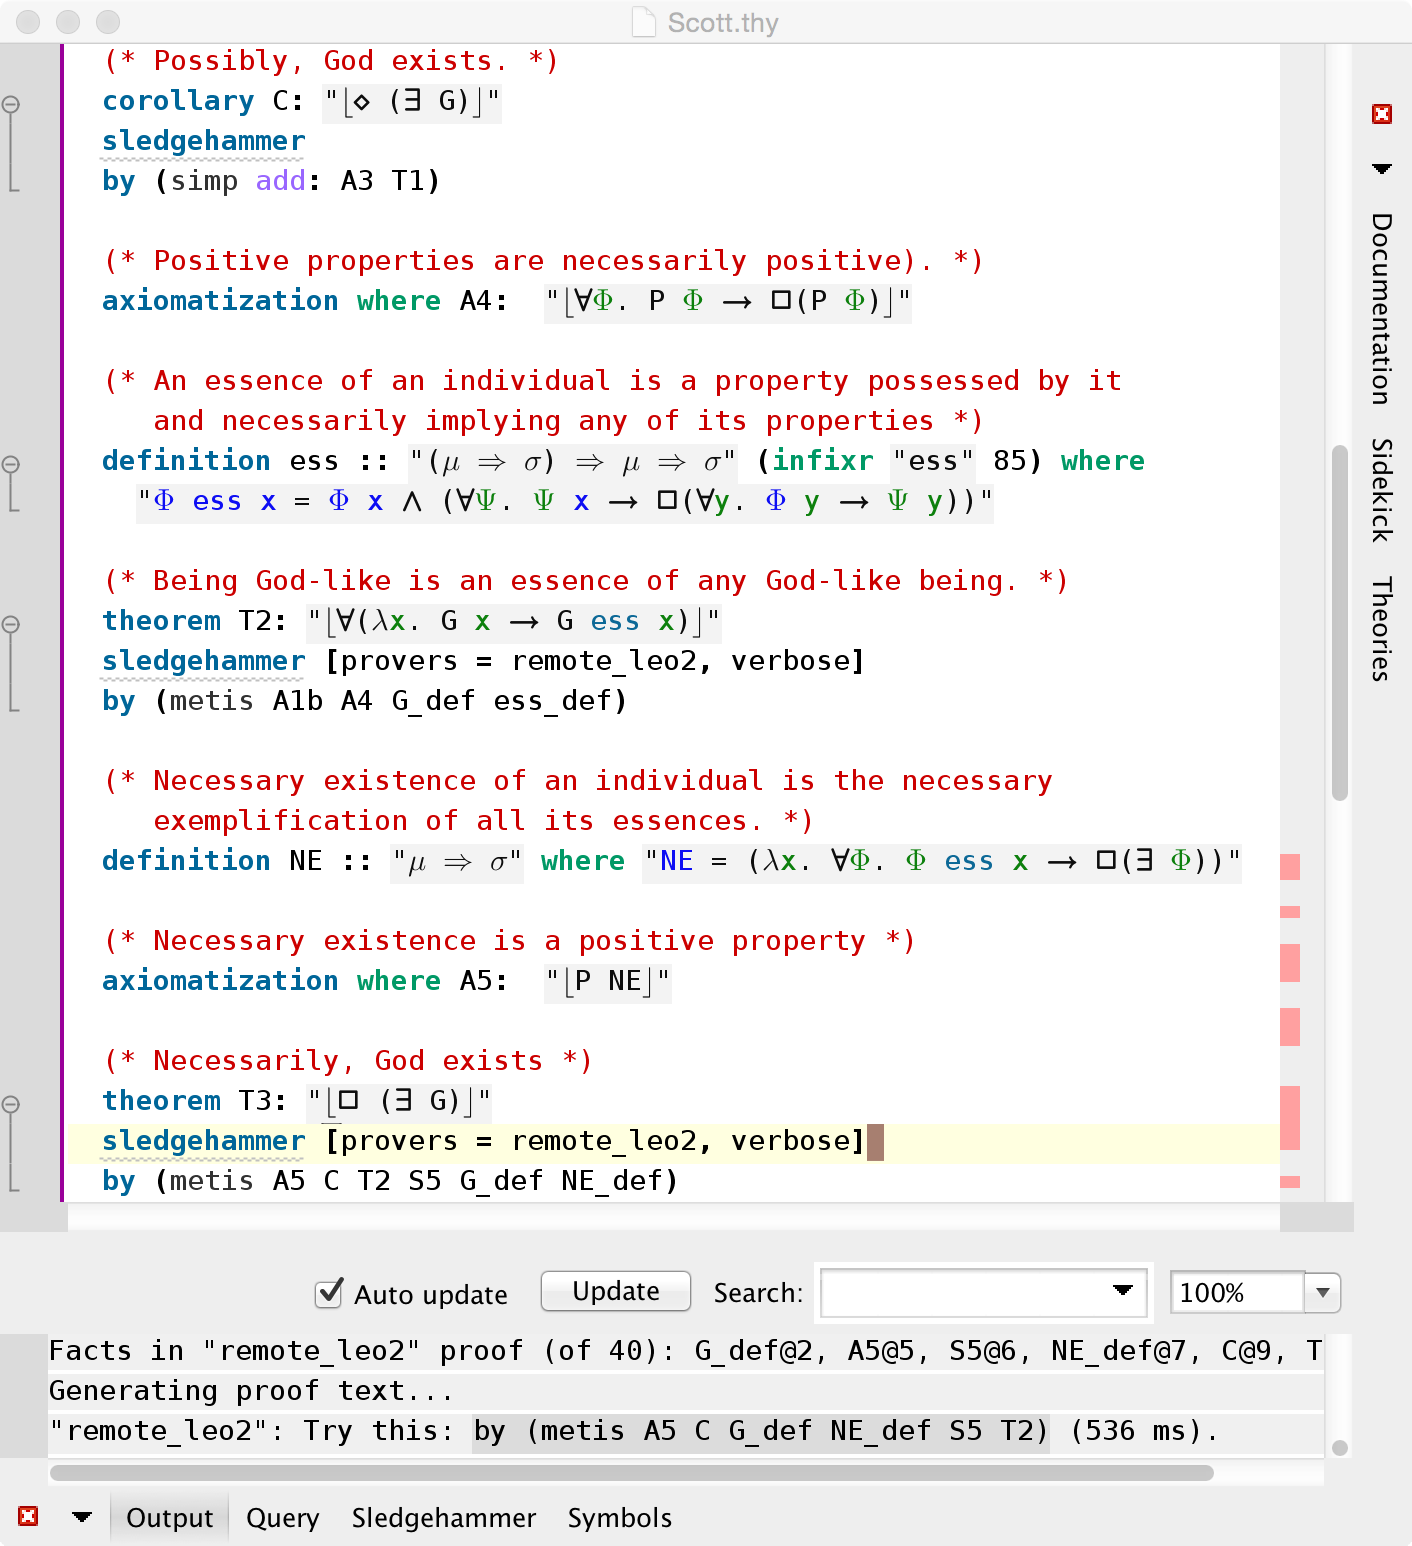
\includegraphics[width=.7\columnwidth]{./Images/Scott.png}}
\caption{File Scott.thy: Dana Scott's variant of G\"odel's Ontological Argument} \label{Scott.thy}
\end{figure}

\subsubsection{Exercise}
The proof in file +Scott.thy+ currently uses logic S5. Try to
experimentally identify the weakest modal logic in which each of the
theorems is provable. Use Nitpick to eventually construct countermodels.


\subsection{Inconsistency of G\"odel's Axioms}
I will report on the discovery and verification of the inconsistency
in G\"odel’s ontological argument with reasoning tools for higher-order
logic. Despite the popularity of the argument since the appearance of
G\"odel’s manuscript in the early 70's, the inconsistency of the axioms
used in the argument remained unnoticed until 2013, when it was
detected automatically by the higher-order theorem prover LEO-II.

Understanding and verifying the refutation generated by LEO-II turned
out to be a time-consuming task. Its completion required the
reconstruction of the refutation in the Isabelle/HOL proof assistant.

The following file contains a rational reconstruction of the
inconsistency argument. We will discuss this file in the tutorial. \\[1em]
+ wget http://www.christoph-benzmueller.de/2016-SFO/Isabelle/Inconsistency_K.thy+\\


\subsection{Actualist versus Possibilist Quantification}
We will study whether changing from constant domain semantics
(possibilist quantification) to
varying domain semantics (actualist quantification) changes the validity of Scott's version of the
ontological argument. First download the following files: \\[1em]
+ wget http://www.christoph-benzmueller.de/2016-SFO/Isabelle/QMLvar.thy+\\
+ wget http://www.christoph-benzmueller.de/2016-SFO/Isabelle/Scottvar.thy+\\

Then inspect the file +QMLvar.thy+ which in addition to what had
before now contains the additional quantifiers $\boldsymbol{\forall}^i$ and
$\boldsymbol{\exists}^i$ (they are restricted to individuals
only). These quantifiers 
realise varying domain semantics as opposed to constant domain
semantics. The old quantifiers remain available as well.

\subsection{Exercise}
At the end of file +QMLvar.thy+ encode instances of the Barcan Formula ($\forall x. \square F(x)
\longrightarrow \Box \forall x. F(x)$; domains cannot grow) and the Converse Barcan
Formula ($\Box \forall x. F(x) \longrightarrow \forall x. \Box F(x)$; domains cannot shrink)
and study their validity within Isabelle/HOL utilising the semantic
embedding approach. Of course, the idea is to employ now the new quantifiers.

\subsection{Exercise}
Can you modify file +QMLvar.thy+  in such a way that we obtain
cumulative domains? Check your attempts with the Barcan Formulas.


\subsection{Scott's Variant in Logic S5 with a Universal Accessibility Relation}
We explore in this part a more efficient way of automating
higher-order modal logic S5 with a universal accessibility
relation. When assuming a universal accessibility
relation the guarding clauses in the definition of the Box and the
Diamond operators can be dropped. 

In Scott's variants, theorem T3 (Necessarily, God exists) can now be proved in a single
step from the axioms in less than 3 seconds.

The relevant files are \\[1em]
+ wget http://www.christoph-benzmueller.de/2016-SFO/Isabelle/QML_S5U.thy+ \\
+ wget http://www.christoph-benzmueller.de/2016-SFO/Isabelle/Scott_S5U.thy+\\
\\[1em]



\section{Multimodal Logics}

\subsection{General Idea}
The idea is to obtain multimodal logics by introducing multiple
accessibility relations and by generalising the Box and Diamond
operator to accept an accessibility relation as first argument. This
way we can introduce indexed box operators.

More details on the embedding of multimodal logics is available here:
\begin{itemize}
\item Combining and Automating Classical and Non-Classical Logics in
  Classical Higher-Order Logic (Christoph Benzm\"uller), In Annals of
  Mathematics and Artificial Intelligence (Special issue Computational
  logics in Multi-agent Systems (CLIMA XI)), volume 62, number 1-2,
  pp. 103-128, 2011. Available at
  \href{http://christoph-benzmueller.de/papers/J25.pdf}{http://christoph-benzmueller.de/papers/J25.pdf}.
\end{itemize}

\subsubsection{Exercise}
Realise this idea by appropriately modifying the file +QML.thy+ from
before.

\subsection{Exercise}
Try to prove the quantified multimodal problems 4--12 from the above article in Isabelle/HOL
using your extended embedding.


\section{Quantified Conditional Logic}
  A notion of quantified conditional logics is studied that
  includes quantification over individual and propositional
  variables. The former is supported with respect to constant and
  variable domain semantics.  A sound and complete
  embedding of this framework in classical higher-order logic is
  presented. Using prominent examples from the literature it is
  demonstrated how this embedding enables effective automation of
  reasoning within (object-level) and about (meta-level) quantified
  conditional logics with off-the-shelf higher-order theorem provers
  and model
  finders. 

Further reading
\begin{itemize}
\item Automating Quantified Conditional Logics in HOL (Christoph
  Benzmüller), In 23rd International Joint Conference on Artificial
  Intelligence (IJCAI-13) (Francesca Rossi, ed.), pp. 746-753, 2013.
  \href{http://christoph-benzmueller.de/papers/C37.pdf}{http://christoph-benzmueller.de/papers/C37.pdf}
\item Cut-Elimination for Quantified Conditional Logic (Christoph
  Benzmüller), In Journal of Philosophical Logic, 2016. (Accepted for
  publication, forthcoming) 

\href{http://christoph-benzmueller.de/papers/J31.pdf}{http://christoph-benzmueller.de/papers/J31.pdf}
\end{itemize}

\subsubsection{Exercise}
Encode the embedding of quantified conditional logic from the above
papers in Isabelle/HOL. You may adapt the file +QML.thy+.

The relevant files are \\[1em]
+ wget http://www.christoph-benzmueller.de/2016-SFO/Isabelle/ConditionalLogic.thy+ \\
\\[1em]

\subsubsection{Exercise}
Encode the Examples 1-5 from the IJCAI paper and prove or refute  them
with Sledgehammer or Nitpick.





\section{Multivalued Logics}
Classical logics are based on the bivalence principle, that is, the
set of truth-values $V$ has cardinality $|V| = 2$, usually with
$V = \{T, F\}$ where $T$ and $F$ stand for truthhood and falsity,
respectively.  Many-valued logics (MVL) generalize this requirement
and allow $V$ to be a more or less arbitrary set of truth-values,
often referred to as \textit{truth-degrees}.  Popular examples of
many-valued logics are fuzzy logics with an uncountable set of
truth-degrees, G\"odel logics and \L ukasiewicz logics with
denumerable sets of truth-degrees, and, from the class of
finitely-many-valued logics, Dunn/Belnap's four-valued logic.
 
Here we study an approach for automating multivalued logics based on a
sixteen-valued lattice, denoted \textit{SIXTEEN}. This system has been
developed by Shramko and Wansing as a generalization of the mentioned
Dunn/Belnap four-valued system to knowledge bases in computer networks
and was subsequently further investigated in various contexts.
 

Further reading:
\begin{itemize}
\item Sweet SIXTEEN: Automation via Embedding into Classical
  Higher-Order Logic (Alexander Steen, Christoph Benzm\''uller), In 7th
  International Conference Non-Classical Logic -- Theory and
  Applications, Toruń, Poland, 2015.  Available at:   \href{http://christoph-benzmueller.de/papers/C49.pdf}{http://christoph-benzmueller.de/papers/C49.pdf}
\item Long paper version (currently submitted) available
  \href{http://christoph-benzmueller.de/papers/2016-Sixteen.pdf}{http://christoph-benzmueller.de/papers/2016-Sixteen.pdf}
\item Slides available at  \href{http://christoph-benzmueller.de/papers/2016-Torun.pdf}{http://christoph-benzmueller.de/papers/2016-Torun.pdf}
\end{itemize}
 
The relevant files are \\[1em]
+ cd ~/LogicEmbeddingsTutorial+\\
+ mkdir MultivaluedLogics+ \\
+ cd MultivaluedLogics+ \\
+ wget http://www.christoph-benzmueller.de/2016-SFO/Isabelle/SIXTEEN.thy+ \\

\subsubsection{Exercise}



\section{Free Logic (Scott)}
Reading:
\begin{itemize}
\item Existence and description in formal logic (Dana Scott),
  1967. Available here: 
  \href{http://journals.cambridge.org/action/displayAbstract?fromPage=online&aid=9103650&fileId=S0022481200077732}{\textbf{here}}
\item Very end of the slides from my  UC Berkeley talk at:
   \href{http://christoph-benzmueller.de/papers/2015-Berkeley.pdf}{http://christoph-benzmueller.de/papers/2015-Berkeley.pdf}.
 % (coming soon)
\end{itemize}


The relevant files are \\[1em]
+ cd ~/LogicEmbeddingsTutorial+\\
+ mkdir FreeLogic+ \\
+ cd FreeLogic+ \\
+ wget http://www.christoph-benzmueller.de/2016-SFO/Isabelle/FreeHOL.thy+ \\





\section{Nominal Logics / Hybrid Logics}
Reading:
\begin{itemize}
\item Embedding of Quantified Higher-Order Nominal Modal Logic into
  Classical Higher-Order Logic (Max Wisniewski, Alexander Steen), 1st
  International Workshop on Automated Reasoning in Quantified
  Non-Classical Logics (ARQNL 2014), Vienna, Austria, Proceedings,
  EasyChair, EasyChair Proceedings in Computing, volume 33,
  pp. 59--64, 2014. Available 
  \href{http://easychair.org/publications/download/Embedding_of_Quantified_Higher-Order_Nominal_Modal_Logic_into_Classical_Higher-Order_Logic}{\textbf{here}}
\item (Section 5.4 of) Higher-Order Modal Logics: Automation and Applications
  (Christoph Benzm\"uller, Bruno Woltzenlogel Paleo), In Reasoning Web
  2015 (Adrian Paschke, Wolfgang Faber, eds.), Springer, LNCS, number
  9203, pp. 32-74, 2015. Available at \href{http://christoph-benzmueller.de/papers/C46.pdf}{http://christoph-benzmueller.de/papers/C46.pdf}
\end{itemize}



\section{Access Control Logics}
Prominent access control logics can be translated in a sound and
complete way into modal logic S4. We have previously outlined how
normal multimodal logics, including monomodal logics K and S4, can be
embedded in simple type theory and we have demonstrated that
higher-order theorem provers can automate reasoning in and about
them. Here we combine these results to provide  a sound (and
complete) embedding of different access control logics in simple type
theory. 

Further reading:
\begin{itemize}
\item Automating Access Control Logic in Simple Type Theory with
  LEO-II (Christoph Benzm\"uller), In Emerging Challenges for Security,
  Privacy and Trust, 24th IFIP TC 11 International Information
  Security Conference, SEC 2009, Pafos, Cyprus, May 18-20,
  2009. Proceedings (Dimitris Gritzalis, Javier López, eds.),
  Springer, IFIP, volume 297, pp. 387-398, 2009. Available at \href{http://christoph-benzmueller.de/papers/C27.pdf}{http://christoph-benzmueller.de/papers/C27.pdf}
\end{itemize}


\section{Zalta's Theory of Abstract Objects}
Reading:
\begin{itemize}
\item Zalta's website: \href{https://mally.stanford.edu/theory.html}{https://mally.stanford.edu/theory.html}
\item Very end of the slides from my  UC Berkeley talk at: % (coming soon)
  \href{http://christoph-benzmueller.de/papers/2015-Berkeley.pdf}{http://christoph-benzmueller.de/papers/2015-Berkeley.pdf}.
\end{itemize}

This is unpublished material; please contact me for further details.

For this theory some further convenient abbreviations are available
(they are already
defined in file +abbrevs+):  mexe, mexe1, mexe2, mexe3, menc, mtop, mbot, mthat, mlam0,
mlam1, mlam, mlam2, mlam3, xt, xp, xf, xe

\begin{tabular}{l|l|l}
shortcut & alternative latex-like input & displayed as \\ \hline
+mneg+ & +\bol\not+ & $\boldsymbol{\neg}$ \\
+mor+ & +\bol\or+ & $\boldsymbol{\vee}$ \\
+mand+ & +\bol\and+ & $\boldsymbol{\wedge}$ \\
+mimpl+ & +\bol\right+ & $\boldsymbol{\rightarrow}$ \\
+mequiv+ & +\bol\leftr+ & $\boldsymbol{\leftrightarrow}$ \\
+mall+ & +\bol\for+ & $\boldsymbol{\forall}$ \\
+mexi+ & +\bol\exi+ & $\boldsymbol{\exists}$ \\
+mnegpred+ &  & ${^\neg}$ \\
+mvalid+ &  +\lf\rf+ & ${\lfloor}\, {\rfloor}$ \\ \hline
+mexe+ &  +(|,|)+ & $\llparenthesis,\rrparenthesis$ \\
+mexe1+ &  +(|,|)+ & $\llparenthesis,\rrparenthesis$ \\
+mexe2+ &  +(|,,|)+ & $\llparenthesis,,\rrparenthesis$ \\
+mexe3+ &  +(|,,,|)+ & $\llparenthesis,,,\rrparenthesis$ \\
+menc+ &  +{|,|}+ & \\
+mequi+ & +\bol\equ+ & $\boldsymbol{\equiv}$ \\
+mthat+ & +\bol\io+ & $\boldsymbol{\iota}$ \\
+mtop+ & +\top+ & $\top$ \\
+mbot+ & +\bot+ & $\bot$ \\
+mlam+ & +\bol\lam+ & $\boldsymbol{\lambda}$ \\
+mlam0+ & & $\boldsymbol{\lambda}^0$ \\
+mlam1+ & & $\boldsymbol{\lambda}^1$ \\
+mlam2+ & & $\boldsymbol{\lambda}^2$ \\
+mlam3+ & & $\boldsymbol{\lambda}^3$ \\
+xt+ & & $x^T$ \\
+xf+ & & $x^F$ \\
+xp+ & & $x^P$ \\
+xe+ & & $x^E$ \\
\end{tabular}


\end{document}